\documentclass{article}
\usepackage[utf8]{inputenc}
\usepackage{geometry}
 \geometry{
 a4paper,
 total={170mm,257mm},
 left=20mm,
 top=20mm,
 }
 \usepackage{graphicx}
 \usepackage{titling}
\usepackage{mathptmx}
\usepackage{amsmath, amsthm, amssymb, calrsfs, wasysym, verbatim, bbm, color, graphics}
\usepackage{float}
\usepackage{longtable}
\usepackage{rotating}
\usepackage{adjustbox}
\usepackage{booktabs}
\usepackage{caption}
\usepackage[english]{babel}
\usepackage[table]{xcolor}
\usepackage{multicol}
\usepackage{hyperref}
\usepackage{amsmath}
\usepackage{listings}
\usepackage{pythonhighlight}
\lstnewenvironment{Python}[1][]{\lstset{style=mypython, frame=none, #1}}{}
 

 \title{Data and Information Quality Project
}
\author{Sofia Martellozzo}
\date{January 2023}
 
 \usepackage{fancyhdr}
\fancypagestyle{plain}{%  the preset of fancyhdr 
    \fancyhf{} % clear all header and footer fields
    \fancyfoot[R]{
\includegraphics[width=1.5cm]{logo_polimi.png}}
    \fancyfoot[L]{\thedate}
    \fancyhead[L]{DQ Project}
    \fancyhead[R]{\theauthor}
}
\pagestyle{plain}
\makeatletter
\def\@maketitle{%
  \newpage
  \null
  \vskip 1em%
  \begin{center}%
  \let \footnote \thanks
    {\LARGE \@title \par}%
    \vskip 1em%
    %{\large \@date}%
  \end{center}%
  \par
  \vskip 1em}
\makeatother

\usepackage{lipsum}  
\usepackage{cmbright}

\begin{document}

\maketitle

\noindent\begin{tabular}{@{}ll}
    Student & \theauthor\\
     StudentID &  996215\\
     Student Personal Code & 10623060\\
      & \\
     Project ID & 18\\
     Assigned Dataset & \texttt{letter.csv}\\
     Assigned Task & Classification
\end{tabular}

%----------------------------------------------------%
\section*{Introduction}
In this project is faced a Classification problem , with two different Machine Learning algorithm, after an imputation of data on the datasets provided, where it encounter NaN values, with two different techniques.\\\\
The dataset is composed of 2001 samples and 17 labels: 'x-box', 'y-box', 'width', 'high’,  'onpix', 'x-bar', 'y-bar', 'x2bar', 'y2bar', 'xybar', 'x2ybr', 'xy2br', 'x-ege', 'xegvy', 'y-ege', 'yegvx' and 'letter' , that is the target  to predict. The values of the different labels are almost all around 0 and 15, while the target are 26 different letters: 'L', 'F', 'Z', 'T', 'U', 'H', 'Y', 'B', 'R', 'O', 'X', 'S', 'M', 'P', 'K', 'Q', 'V', 'C', ‘W’,  'N', 'G', 'J', 'E', 'A', 'I', 'D' .

%---------------------------------------------------%
\section{Setup choices}

\subsection{Chosen ML algorithm}\label{sec:model}
Supervised learning learns a function to make prediction of a defined label based on the input data. It can be either classifying data into a category (classification problem) or forecasting an outcome (regression algorithms).\\
Classification model identifies which category an object belongs to whereas regression model predicts a continuous output. Sometimes there is an ambiguous line between classification algorithms and regression algorithms.\\
Many algorithms can be used for both classification and regression, and classification is just regression model with a threshold applied. When the number is higher than the threshold it is classified as true while lower classified as false. \\\\
Here follows the description of the two ML algorithm selected to solve the Classification problem on the {\texttt letter} dataset.

\subsubsection*{Support Vector Classifier (SVC)}
\begin{multicols}{2}
\begin{figure}[H]
        \begin{center}
        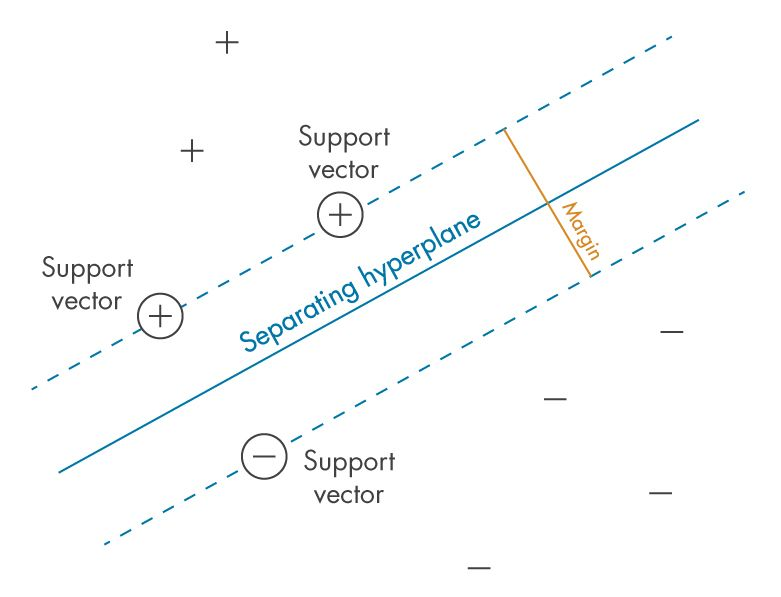
\includegraphics[width=0.4\textwidth]{SVC.jpeg}
        \end{center}
    \end{figure} 
    \columnbreak
\columnbreak
Support Vector Classifier (SVC) is developed based on Support Vector Machine (SVM): a type of deep learning algorithm, builds a learning model that assigns new examples to one group or another. By these functions, SVMs are called a non-probabilistic, binary linear classifier. SVM finds the best way to classify the data based on the position in relation to a border between positive class and negative class. This border is known as the hyperplane which maximize the distance between data points from different classes.
\end{multicols}
\begin{center}
How is implemented in python:
\begin{Python}
from sklearn.svm import SVC
svc = SVC()
svc.fit(X_train, y_train)
y_pred = svc.predict(X_test)
\end{Python}
\end{center}


\newpage
\subsubsection*{Decision Tree Classifier}
\begin{multicols}{2}
A decision tree is a flowchart-like tree structure where an internal node represents feature(or attribute), the branch represents a decision rule, and each leaf node represents the outcome. It partitions the tree in recursively manner call recursive partitioning. This flowchart-like structure helps you in decision making.\\Decision Tree is a white box type of ML algorithm. It shares internal decision-making logic, which is not available in the black box type of algorithms such as Neural Network. Its training time is faster compared to the neural network algorithm.\\ Decision tree builds tree branches in a hierarchy approach and each branch can be considered as an if-else statement. The branches develop by partitioning the dataset into subsets based on most important features. Final classification happens at the leaves of the decision tree.
 \columnbreak
\begin{figure}[H]
        \begin{center}
        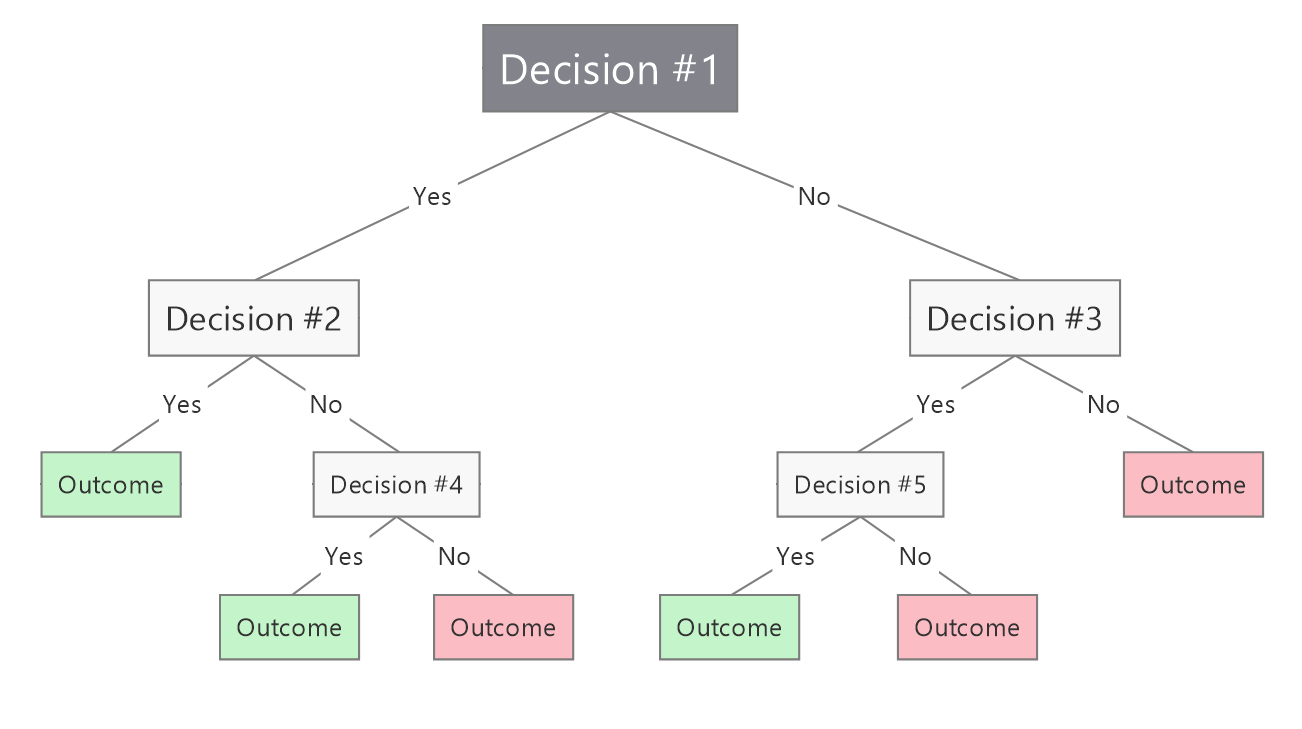
\includegraphics[width=0.5\textwidth]{DecTree.png}
        \end{center}
    \end{figure} 
\end{multicols}
\begin{center}
    How is implemented in python:
\begin{Python}
from sklearn.tree import DecisionTreeClassifier
dtc = DecisionTreeClassifier()
dtc.fit(X_train, y_train)
y_pred = dtc.predict(X_test)
\end{Python}
\end{center}

%----------------------------------------------------%

\subsection{Chosen ML performance evaluation metrics} \label{sec:performances}
In this section is provided a simple description of different metrics used to evaluate the performance of the algorithms developed for the classification. 

\subsubsection*{Confusion Matrix}
A confusion matrix is an extremely useful tool, used to define the performance of a classification algorithm, especially in multi-class classification problems. It is a matrix that compares the number of predictions for each class that are correct and those that are incorrect. Each row of the matrix represents the instances in a predicted class, while each column represents the instances in an actual class (or vice versa).\\ The name stems from the fact that it makes it easy to see if the system is confusing two classes (i.e. commonly mislabeling one as another).  
In a confusion matrix, there are 4 numbers to pay attention to:
\begin{itemize}
    \item True positives: The number of positive observations the model correctly predicted as positive.
    \item False positive: The number of negative observations the model incorrectly predicted as positive.
    \item True negative: The number of negative observations the model correctly predicted as negative.
    \item False negative: The number of positive observations the model incorrectly predicted as negative.
\end{itemize}
An example of confusion matrix in this project is as follows:
\begin{figure}[H]
        \begin{center}
        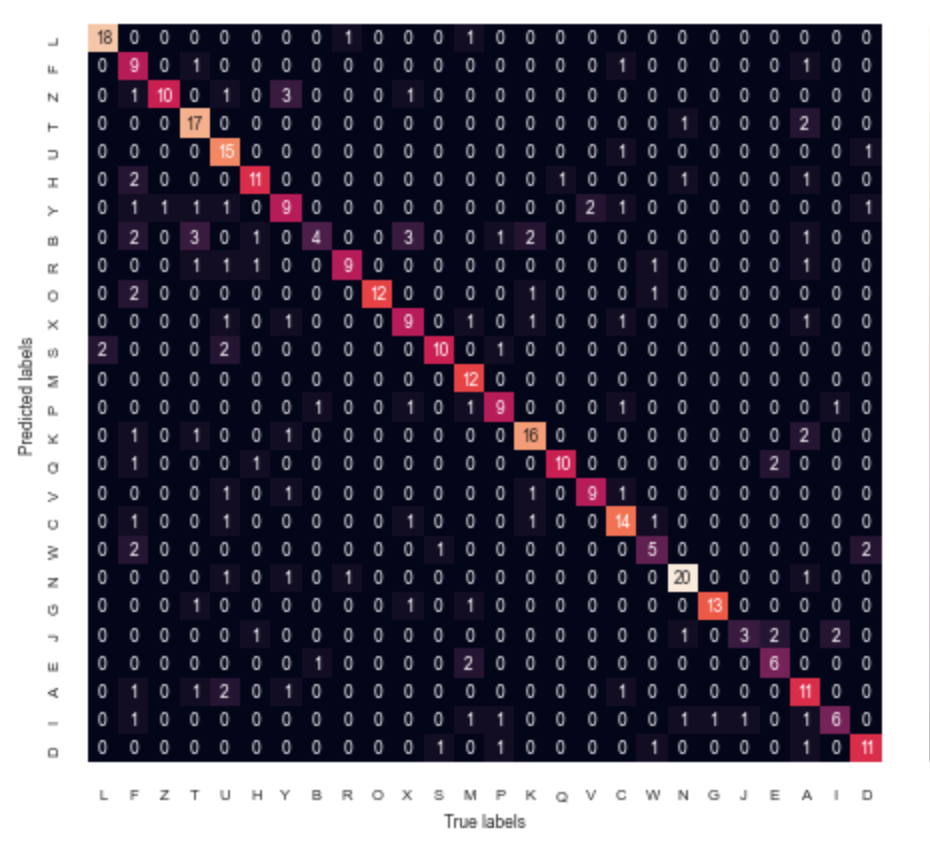
\includegraphics[width=0.33\textwidth]{cm.png}
        \end{center}
\end{figure} 

\subsubsection*{Accuracy}
The overall accuracy of a model is simply the number of correct predictions divided by the total number of predictions. An accuracy score will give a value between 0 and 1, a value of 1 would indicate a perfect model.
\begin{center}
    \begin{math}
Accuracy = \frac{\mbox{Correct Prediction}}{\mbox{Total Predictions}}
\end{math}
\end{center}
It is calculated on all the predicted value (overall accuracy of the model) and also specifically on each label predicted. 

\subsubsection*{Precision}
Precision measures how good the model is at correctly identifying the positive class. In other words out of all predictions for the positive class how many were actually correct?
\begin{center}
    \begin{math}
        Precision = \frac{\mbox{True Positive}}{\mbox{True Positive} + \mbox{False Positive}}
    \end{math}
\end{center}

\subsubsection*{Recall}
Recall tell us how good the model is at correctly predicting all the positive observations in the dataset. However, it does not include information about the false positives. 
\begin{center}
    \begin{math}
        Recall = \frac{\mbox{True Positive}}{\mbox{True Positive} + \mbox{False Negative}}
    \end{math}
\end{center}
Usually, precision and recall are observed together. 

\subsubsection*{F1-score}
The F1 score is the harmonic mean of precision and recall. The F1 score will give a number between 0 and 1. If the F1 score is 1.0 this indicates perfect precision and recall. If the F1 score is 0 this means that either the precision or the recall is 0.
\begin{center}
    \begin{math}
        F1-score =\quad \mbox{2} x \quad\dfrac{\mbox{Precision} x \mbox{Recall}}{\mbox{Precision} + \mbox{Recall}} 
    \end{math} 
\end{center}





%---------------------------------------------------%
\subsection{Imputation techniques selected}
Imputation is a technique used to handle missing values in a dataset. It involves replacing missing values with estimated ones, in order to make the data usable for analysis or modeling. There are several imputation techniques that can be used, depending on the nature of the data and the purpose of the analysis.
\subsubsection*{Mode Imputation}
This technique replaces the missing value with the mode of the non-missing values in the same column. It is a simple and straightforward method, but it can introduce bias in the data if the missing values are not missing at random. The steps to perform mode imputation are:
\begin{enumerate}
    \item Identify the missing values in the dataset.
    \item Compute the mode of the feature for the non-missing values.
    \item Replace the missing value with the computed mode.
\end{enumerate}
Mode imputation is a good choice when the data has a large number of observations for the mode. However, when the data is not missing completely at random, mode imputation can introduce bias into the data and can be misleading. It is important to note that this method will only work when the variable is categorical or ordinal, if the variable is continuous it will not work. 

\subsubsection*{K-Nearest Neighbors (KNN) Imputation}
It is a form of sample imputation that uses the values of similar cases to fill in the missing data. The idea behind KNN imputation is that a point value can be estimated by the average or the mode of the k-nearest points where k is a user-specified parameter. The steps to perform KNN imputation are:
\begin{enumerate}
    \item Identify the missing values in the dataset.
    \item For each missing value, find the k-nearest neighbors based on a distance metric, such as Euclidean distance.
    \item Compute the average or the mode of the feature of the k-nearest neighbors.
    \item Replace the missing value with the computed average or mode.
\end{enumerate}
KNN imputation is a non-parametric method, which means that it does not make any assumptions about the underlying distribution of the data.\\
It is important to note that the choice of k is crucial for the performance of the KNN imputation. If k is too small, the imputed values will be very sensitive to the presence of outliers, if k is too large, the imputed values will be too similar to the overall mean of the variable.\\
Since in this case no outliers are present in the dataset, the choice of k end up in a small value: exactly 5.\\\\
It is important to notice that imputation can introduce bias into the data, so it is important to evaluate the performance of the imputation method and the impact on the analysis or model.


%---------------------------------------------------%
\section{Pipeline implementation}
Here is explained step by step, how t
\begin{enumerate}
    \item After downloaded the dataset in the Anaconda environment, it is explored to better understand what it countains. As said before it countains 2001 sample of 25 different integer feature and a label, that is a letter.
    \item \begin{multicols}{2}
    A histogram is a graphical representation of the distribution of a dataset. It is a way to visualize the frequency of different values in a dataset. In the case of the 'letter' column, a histogram shows the frequency of each letter in the column.\\ Additionally, you can also see if the data is balanced or imbalanced. A balanced dataset would have similar frequencies for each letter, while an imbalanced dataset would have some letters that appear more frequently than others.\\From the image reported on the right is possible to see that this dataset is not much imbalanced.
        \columnbreak
        \begin{figure}[H]
            \begin{center}
            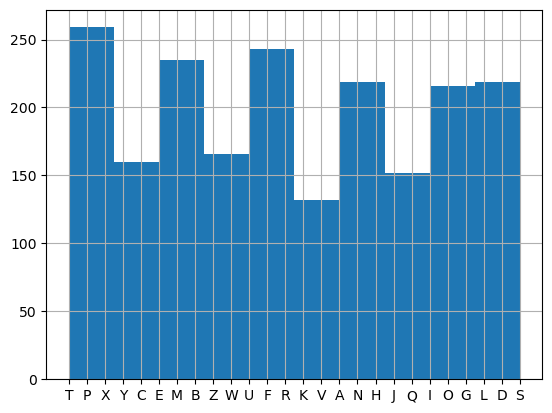
\includegraphics[width=0.34\textwidth]{histogram.png}
            \caption{Histogram of targets}
            \end{center}
        \end{figure} 
    \end{multicols}
    \item \begin{multicols}{2}A grouped by chart, also known as a grouped bar chart or a grouped column chart, is a type of chart that is used to compare the values of different categories within a dataset. It is typically used to compare the values of a single variable across different groups or categories.\\A grouped by chart is similar to a regular bar chart or column chart, but instead of having one bar or column for each data point, it has multiple bars or columns for each data point, grouped together by category.\\Grouped by chart are useful for showing the relationship between multiple variables, especially when the values are being compared across several groups or categories.
    \columnbreak
    \begin{figure}[H]
            \begin{center}
            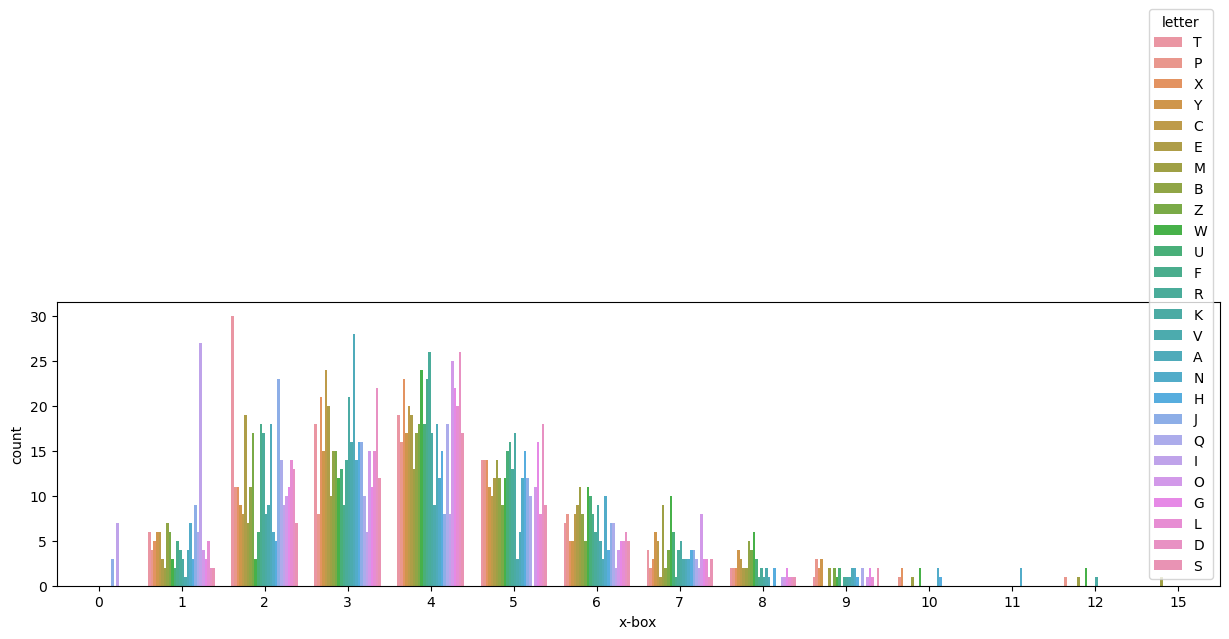
\includegraphics[width=0.4\textwidth]{gbychart.png}
            \caption{Grouped by chart of 'count' feature}
            \end{center}
        \end{figure} 
    \end{multicols}
    \item \begin{multicols}{2}A box plot, also known as a box-and-whisker plot, is a graphical representation of a dataset that shows the distribution of the data. It is a way to visualize the spread and skewness of the data.\\A box plot consists of a box, which represents the interquartile range (IQR) of the data, and whiskers, which extend from the box to show the full range of the data. The box represents the middle 50\% of the data, and the whiskers represent the full range of the data.\\
    In this dataset the values vary significally between the different feature for the different label. 
    \columnbreak
    \begin{figure}[H]
            \begin{center}
            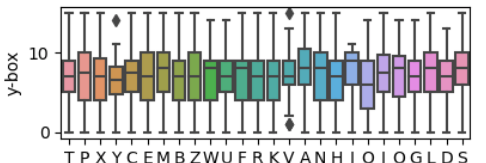
\includegraphics[width=0.4\textwidth]{boxplot.png}
            \caption{Box Plot for 'y-box' feature}
            \end{center}
        \end{figure}    
    \end{multicols} 
    \item At first inject randomly, in the original dataset provided, some NaN values, with the script provided.
    \item Save in two list a copy of the 5 different dirty dataset generated, each list for each imputation technique. Each dataset differentiate from the original one by the percentage of null values: 50\%, 40\%, 30\%, 20\%, 10\% .
    \item Apply both the two imputation technique on all the generated dataset, in order to achive a completeness of 100\%. 
    \item Evaluate the imputation techniques by calculating the accuracy, comparing the generated datasets with the original one.
    \item Split all the 10 datasets in Train and Test set, with the function provided by the library \texttt{from sklearn.model\_selection}
    \item Perform the classification on all the datasets with the two algorithm chosen: SVC and Decision Tree Classifier (explained in \ref{sec:model})
    \item Evaluate the performance of the ML algorithm on the results obtained \ref{sec:performances}
\end{enumerate}


%---------------------------------------------------%
\section{Results}
Concerning the Imputation techniques the results obtained are the following:\\\\
Mode Imputation:
\begin{center}
    \begin{table}[h]
\begin{tabular}{|c|c|c|c|c|c|c|c|c|c|}
\hline
 & x-box & y-box & width & high & onpix & x-bar & y-bar & x2bar & y2bar \\ \hline
dataset1 & 61.7\% & 56.3\% & 61.0\% & 59.8\% & 58.8\% & 64.1\% & 65.5\% & 59.2\% & 58.0\% \\ \hline
dataset2 & 69.1\% & 65.2\% & 67.8\% & 65.0\% & 68.5\% & 72.2\% & 72.4\% & 68.0\% & 67.0\% \\ \hline
dataset3 & 76.7\% & 72.7\% & 77.8\% & 74.0\% & 75.9\% & 80.9\% & 81.4\% & 73.3\% & 77.0\% \\ \hline
dataset4 & 84.4\% & 83.3\% & 84.6\% & 83.6\% & 83.5\% & 85.0\% & 86.1\% & 83.7\% & 83.8\% \\ \hline
dataset5 & 91.8\% & 91.6\% & 92.4\% & 91.8\% & 92.1\% & 93.5\% & 93.2\% & 90.7\% & 91.4\% \\ \hline
\end{tabular}
\end{table}

\begin{table}[h]
\begin{tabular}{|c|c|c|c|c|c|c|c|c|c|}
\hline
 & xybar & x2ybr & xy2br & x-ege & xegvy & y-ege & yegvx & total \\ \hline
dataset1 & 62.8\% & 64.6\% & 67.2\% & 61.3\% & 70.6\% & 59.9\% & 68.5\% & 62.5\% \\ \hline
dataset2 & 71.5\% & 71.6\% & 72.1\% & 69.6\% & 74.8\% & 65.9\% & 76.0\% & 69.8\% \\ \hline
dataset3 & 77.5\% & 79.2\% & 79.5\% & 77.4\% & 82.4\% & 75.5\% & 82.0\% & 77.7\% \\ \hline
dataset4 & 85.4\% & 85.0\% & 86.1\% & 83.6\% & 88.6\% & 84.2\% & 87.7\% & 84.9\% \\ \hline
dataset5 & 92.5\% & 92.8\% & 92.4\% & 91.5\% & 93.7\% & 92.1\% & 93.9\% & 92.3\% \\ \hline
\end{tabular}
\end{table}
\end{center}
The best result is obtained in the first dataset (the one with 50\% of completeness) since, with the imputation are injected 12.5\% of correct values, generating a dataset of 62.5\% of accuracy in the hole. Not taking into account the initial condition of the data, this score is not a really good one, it contains a significant number of wrong data.\\\\
KNN Imputation:
\begin{center}
    \begin{table}[h]
\begin{tabular}{|c|c|c|c|c|c|c|c|c|c|}
\hline
& x-box & y-box & width & high & onpix & x-bar & y-bar & x2bar & y2bar \\ \hline
dataset1 & 52.3\% & 50.5\% & 52.0\% & 52.3\% & 51.5\% & 51.2\% & 54.4\% & 52.4\% & 51.7\% \\ \hline
dataset2 & 62.4\% & 60.7\% & 61.8\% & 60.5\% & 62.7\% & 63.8\% & 63.5\% & 62.5\% & 63.9\% \\ \hline
dataset3 & 72.0\% & 69.8\% & 74.4\% & 71.1\% & 72.8\% & 73.7\% & 75.0\% & 69.8\% & 73.2\% \\ \hline
dataset4 & 81.8\% & 81.8\% & 82.5\% & 81.2\% & 82.2\% & 80.9\% & 82.6\% & 82.0\% & 82.1\% \\ \hline
dataset5 & 90.7\% & 90.9\% & 90.5\% & 90.3\% & 91.7\% & 91.9\% & 91.3\% & 90.1\% & 91.0\% \\ \hline
\end{tabular}

\begin{tabular}{|c|c|c|c|c|c|c|c|c|c|}
\hline
& xybar & x2ybr & xy2br & x-ege & xegvy & y-ege & yegvx & total \\ \hline
dataset1 & 50.3\% & 51.6\% & 54.3\% & 51.1\% & 55.5\% & 53.0\% & 53.4\% & 52.3\% \\ \hline
dataset2 & 61.7\% & 61.6\% & 62.0\% & 62.9\% & 63.5\% & 61.1\% & 64.3\% & 62.4\% \\ \hline
dataset3 & 72.3\% & 72.3\% & 73.2\% & 73.2\% & 74.6\% & 72.6\% & 74.4\% & 72.8\% \\ \hline
dataset4 & 81.8\% & 81.1\% & 82.0\% & 81.7\% & 85.6\% & 82.5\% & 82.9\% & 82.2\% \\ \hline
dataset5 & 90.2\% & 92.1\% & 91.2\% & 91.2\% & 92.2\% & 92.1\% & 92.5\% & 91.2\% \\ \hline
\end{tabular}
\end{table}
\end{center}
In this case the technique performs worst, imputing just a 2\% of correct data.





description of the main result obtained\\
b.	ML performance comparison between the imputation techniques you have implemented



\end{document}
